\subsection{溶液的处理}
%Generated by OCR
%To be fixed
溶液是水溶性晶体生长的母体,溶液状态几乎是先天地决定了晶体生长特性和长成的晶体质量以及培养晶体工作的成败。溶液处理的目的是使溶液高度纯净,减少有害杂质的污染,提高其稳定性,通常制备溶液的步骤是用试剂级原料和蒸馏水或离子交换水配制成一定温度下的饱和溶液,用微米级以下孔径的过滤器过滤,然后在结晶器中过热,冷却到略高于饱和温度即可下籽晶使用。有时根据需要在溶液过滤前还可作调整pH值和掺质等处理。

培养高光学质量的晶体,按上述操作处理溶液往往还达不到要求,下面以培养KDP晶体为例,对培养晶体的溶液如何进行特别处理作一介绍。

KDP晶体作为高功率激光倍频材料,抗光损伤能力是一个很重要的参数。按一般条件培养出来的晶体,其抗光损伤这个参数值是不高的,满足不了应用的需要。经过原料提纯,清除碳化物,灭菌,超细过滤,甚至在生长晶体时对溶液作不间断的连续过滤等特殊处理,使KDP晶体抗光损伤能力有了成倍的提高。

\begin{figure}[htbp]
 \centering
 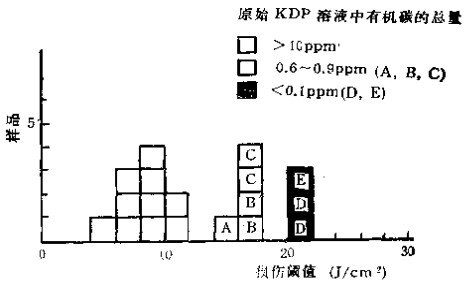
\includegraphics[width=0.8\textwidth]{fig/cp03/img3.30.jpg}
 \caption{溶液特殊处理与晶体光损伤阈值之间的关系:}
\end{figure}

市售分析纯KDP试剂含有较高量无机和有机杂质,必须作化学的和重结晶的提纯处理,杂质在晶体和溶液中的分配系数是不同的,有的容易进入晶体,有的大部分留在溶液中,在重结晶时,采取“去头去尾”的方法是有效的,即重结晶最初析出的固体和最后的母液都弃去不要,只取中间部分产品。原料纯化要特别注意$\rm Fe^{3+}$。$\rm Cr^{3+}$,$\rm Al^{3+}$等高价金属离子,它们不仅影响晶体习性,还影响晶体的光学性质。原料中的有机杂质是通过向溶液中通$\rm O_3$或加$\rm H_2O_2$来清除的。溶液中碳的含量明显与光损伤阈值有关(图3.30)。细菌和微生物是另一类有害污染物质,在晶体生长过程中,这类污染物质在溶液中繁殖增多,为了断绝其繁衍途径,必须对溶液进行消毒处理,用紫外灯辐照,氧化剂氧化和杀菌剂(如汞)灭菌都可以达到此目的。消毒处理应当在晶体生长的全过程中进行。溶液中的机械微粒不仅容易成为异质成核的核心,影响溶液的稳定性,而且容易长入晶体,影响晶体的光学均匀性。特别是某些胶体尺寸的微粒对晶伟生长危害更大,对溶液进行超细过滤,用孔径为0.05$\rm\mu m$的滤膜连续不断地过滤生长晶体中的溶液,可以显著地改善这种状况。

此外,配制溶液和原料重结晶提纯时应十分注意结晶物质的分解温度,过高的温度或局部过热都会导致结晶物质的部分分解,造成新的污染,这对微量杂质即可产生晶体异常生长的场合,对此应特别小心。